\documentclass[10pt,a4paper]{article}
\usepackage[utf8]{inputenc}
\usepackage{amsmath}
\usepackage{amsfonts}
\usepackage{amssymb}
\usepackage{graphicx}
\usepackage{subfigure}
\usepackage{amsmath}
\usepackage{mathrsfs}
\DeclareRobustCommand{\orderof}{\ensuremath{\mathcal{O}}}
\bibliographystyle{prsty}
\usepackage[top=1in, bottom=1in, left=1in, right=1in]{geometry}

\begin{document}
\section{Introduction}
\textbf{chn} is a task of application level. It calculate the Chern number of the system. This task uses the method introduced by JPSJ 74.1674 (2005). Since this method only applies for type-A\footnote{For definition, see the periodic table of topological insulators and superconductors shown in Rev. Mod. Phys. 82 3045} Chern insulator, it only works to 2D system. Because the calculated results are too large, not all data are attached in this file. Also, since NiO is not a 2D structure, so the Haldane\_chn.plb (can be found in examples) is used instead. This code cannot determine whether the band structure if an insulator or not, so one should confirm it before calculating Chern number.  

\section{Dictionary}

\subsection{Input}
\textit{\textbf{chn.Mesh}} This parameter tells PiLab how to mesh the k-space. The method of this code usually doesn't require very dense grids. So you can gradually increase this parameter form small values, say [5,5], to see if the the Chern number converges.\\ \\
\textit{\textbf{chn.DiffVal}}  This parameter tells PiLab how to avoid divergent k-point. In the calculation method, it is possible to have lattice field divergent even if there is no degeneracy. To avoid this issue, one should input a small difference $\textbf{k}  \rightarrow \textbf{k}+ \delta \cdot \textbf{k}^{'}$ to avoid the divergence,where $\delta$ is a small value and $\textbf{k}^{'}$ is an arbitrary vector. Here, DiffVal gives $\delta$ and DiffVec gives $\textbf{k}^{'}$.\\ \\
\textit{\textbf{chn.DiffVec}} See chn.DiffVal    
\subsection{Output}
\textit{\textbf{chn.tot\_Chern}} This variable shows the total Chern number below Fermi level. It must be an integer.\\ \\
\textit{\textbf{chn.HOMO\_ind}} This variable shows which band is the highest occupied band. \\ \\
\textit{\textbf{chn.ban\_Chern}} This variable shows the Chern number of each band. \\ \\
\textit{\textbf{chn.lat\_field}} This variable is the lattice field of each band at each k-point.If there are 10 bands with 25 k-points, this variable will be a 10x25 matrix. The lattice field is a quantity in this method. It can be regarded as the sum of the Chern number of a grid in the k-space contributed form a particular band.  

\begin{figure}[tbp]
\centering
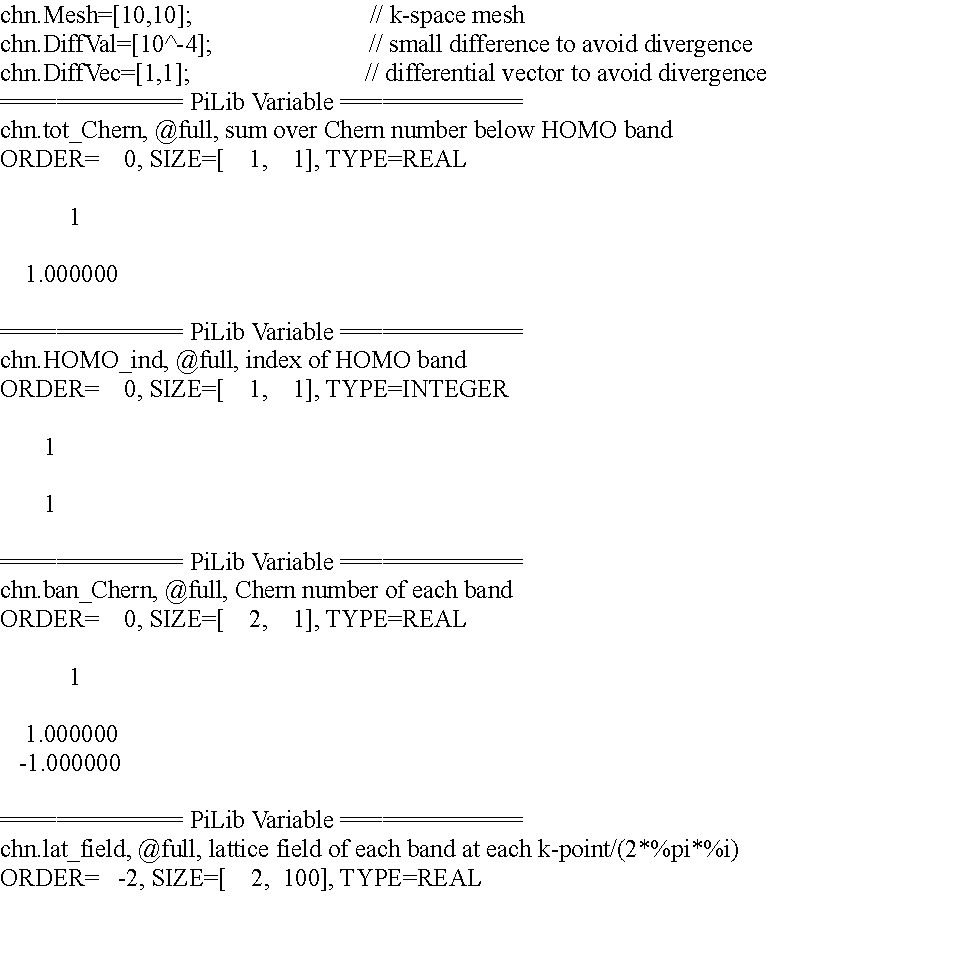
\includegraphics[width=0.9\columnwidth]{Haldane_chn.pdf}
\caption{Haldane\_chn.plb}
\end{figure}

\end{document}